\documentclass[]{article}
\usepackage{amsmath}
\usepackage{amsfonts}
\usepackage{amssymb}
\usepackage{algorithmic}
\usepackage{algorithm}
\usepackage{tikz}
\usepackage{graphicx}
\usepackage{mdframed}
\usepackage{paralist}
\usepackage{listings}

\definecolor{dkgreen}{rgb}{0,0.6,0}
\definecolor{gray}{rgb}{0.5,0.5,0.5}

\lstset{
  language=Python,
  breaklines=true,
  showstringspaces=false,
  frame=single,
  aboveskip=3mm,
  belowskip=3mm,
  columns=flexible,
  basicstyle={\small\ttfamily},
  numbers=none,
  numberstyle=\tiny\color{gray},
  keywordstyle=\color{blue},
  commentstyle=\color{gray},
  stringstyle=\color{dkgreen},
  breakatwhitespace=true,
  tabsize=3
}

\title{CAGD - Homework 5}
\author{Josefine St{\aa}l \& Erik Ackzell}

\begin{document}

\maketitle

\section*{Task 1}
In this task we convert between barycentric and homogeneous coordinates.\\
Consider the points \begin{equation*}
p_0 = \left(\begin{array}{c}
1\\
1\\
1
\end{array}\right), \quad
p_1 = \left(\begin{array}{c}
3\\
3\\
3
\end{array}\right), \quad
p_2 = \left(\begin{array}{c}
1\\
2\\
2
\end{array}\right)
\end{equation*}
and let \begin{equation*}
q_1=\left(\begin{array}{c}
0.25\\
0.25\\
0.5
\end{array}\right)
\end{equation*}
in barycentric coordinates with respect to $p_0, p_1, p_2$. We want to express $q_1$ in homogeneous coordinates.\\
First, we express $q_1$ in Cartesian coordinates \begin{equation*}
q_1 = 0.25p_0 + 0.25p_1 + 0.5p_2 = \left(\begin{array}{c}
0.25 + 1.5 + 0.25\\
0.25 + 1.5 + 0.5\\
0.25 + 1.5 + 0.5
\end{array}\right) = \left(\begin{array}{c}
2\\
2.25\\
2.25
\end{array}\right).
\end{equation*}
For any $\omega\in\mathbb{R}$, the homogeneous coordinates of $q_1$ are\begin{equation*}
q_1 = \left(\begin{array}{c}
2\omega\\
2.25\omega\\
2.25\omega\\
\omega
\end{array}\right),
\end{equation*}
which is what we wanted to show.\\
Now let \begin{equation*}
q_2 = \left(\begin{array}{c}
5\\
4\\
4\\
3
\end{array}\right)
\end{equation*}
in homogeneous coordinates. We wish to express $q_2$ in barycentric coordinates with respect to $p_0, p_1, p_2$.\\
First, we express $q_2$ in Cartesian coordinates \begin{equation*}
q_2 = \left(\begin{array}{c}
\frac{5}{3}\\
\frac{4}{3}\\
\frac{4}{3}
\end{array}\right).
\end{equation*}
We now want to determine the coefficients $a_0, a_1, a_2$ such that \begin{equation*}
\sum_{i=0}^{2}a_ip_i
\end{equation*}
and \begin{equation*}
\sum_{i=0}^{2}a_i=1.
\end{equation*}
This can be done by solving the linear equation system \begin{equation*}
\left(\begin{array}{ccc}
1 & 3 & 1\\
1 & 3 & 2\\
1 & 1 & 1
\end{array}\right)\left(\begin{array}{c}
a_0\\
a_1\\
a_2
\end{array}\right) = 
\end{equation*}
%\begin{figure}[h!]
%	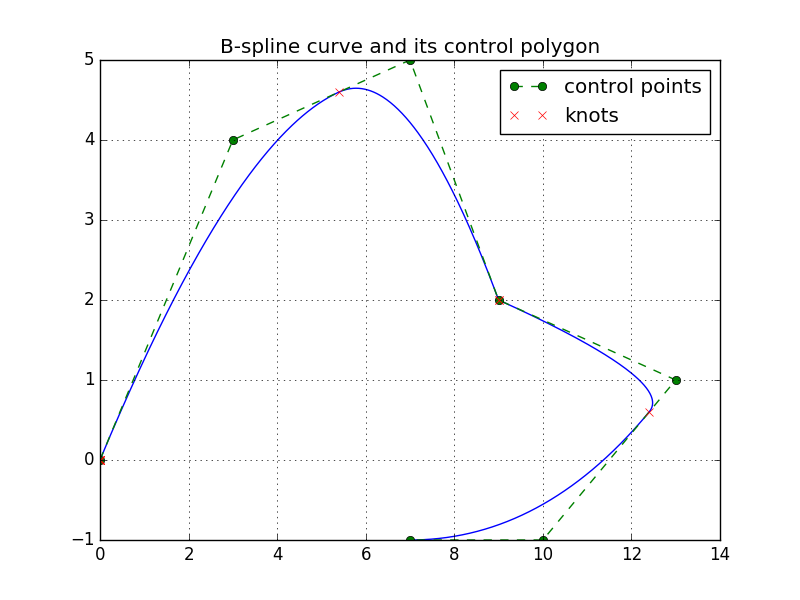
\includegraphics[scale=0.6]{bspline}
%\end{figure}


\newpage
\section*{Appendix I}
%\lstinputlisting[lastline=87]{bsplines.py}

\end{document}
